\documentclass{article}
\usepackage[utf8]{inputenc}
\usepackage[numbers]{natbib}
\usepackage{amsmath}
\usepackage{url}
\usepackage{graphicx}
\usepackage{floatrow}
\usepackage{pdfpages}
\usepackage{csvsimple}
\usepackage{tikz}
\usepackage{pgfplots}
\usepackage{filecontents}

\author{Joris Damian Morger, Nicolas Manuel Alessandro Gagliani, IT12T}

\title{Zweikörpersysteme - Auftrag PSIT HS 2013}

\begin{document}
	\maketitle

	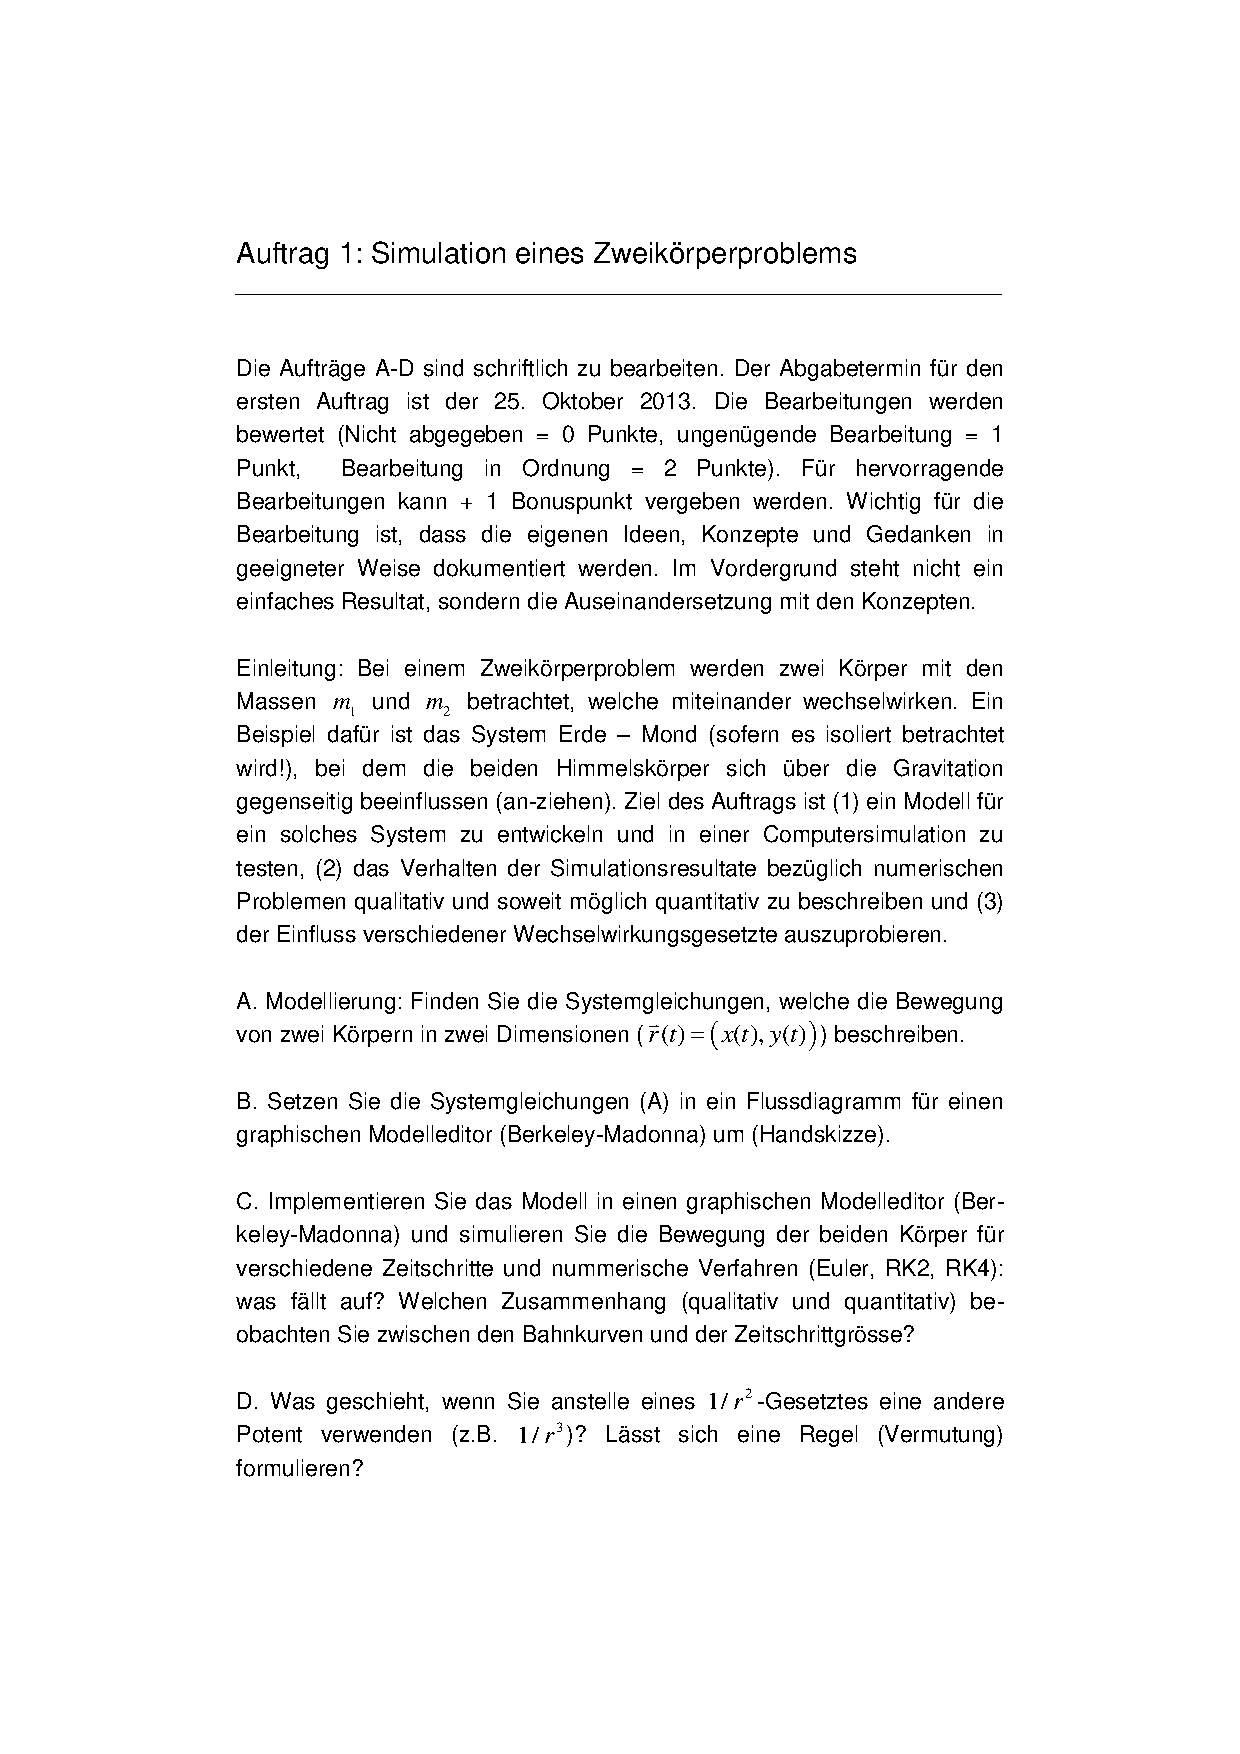
\includepdf[pages={1}]{PhITAuftr1.pdf}

	\section*{Intro}

	Wir betrachten im folgenden zwei isolierte Körper Erde und Mond mit den Massen $m_{Mond}$ und $M_{Erde}$, wobei der Mond in ellipsenförmig um die Erde rotiert.
	Per Definition:
	$$m_{\text{M}} = 7.35 \times 10^{22} \text{ kg} \cite{wiki1}$$

	$$m_{\text{E}} = 5.79 \times 10^{24} \text{ kg} \cite{wiki1}$$

	$$r_{\text{ME}} (Abstand) = 3,844 \cdot 10^8 \text{ m} \cite{wiki2}$$

	$$\gamma = 6.6742^{-11} \frac{Nm^{2} }{kg^2 }$$


	\section*{Teil A}
	\subsection{Fixer Radius}
	Erde und Mond ziehen sich an. Die Kraft zwischen den beiden Massen lässt sich wie folgt berechnen.

	Wir wissen:

	$$T = 27,3217d \approx 2360594s$$
	$$\omega = \frac{2\pi}{T}$$
	$$F_{Z} = m\omega^2r$$

	Daher:
	$$\omega_\text{M} = \frac{2\pi}{T} = \frac{2\pi}{27,3217d} = \frac{2\pi}{2360594s} \approx 2.66\cdot10^{-6} s^{-1}$$
	$$F_\text{Z} = m_\text{M} \cdot \omega_\text{M}^2 \cdot r_\text{ME} \approx 2 \cdot 10^{20} N$$

	$$F_\text{E,M} = \gamma \cdot \frac{{m_\text{E} \cdot m_{\text{M}}}}{{{|{\vec{r_{ME}}}}|^2}}} \cdot \vec{n} \approx -2 \cdot 10^{20} N$$

	Aha! Da die Zentripedalkraft vom Mond und die Gravitationskraft zwischen Mond und Erde die gleiche ist, einfach mit anderem Vorzeichen (also Kraft in andere Richtung), erkennen wir das der Mond und die Erde sich in Balance halten. Sie prallen weder aufeinander, noch bewegen sie sich voneinander weg.

	\subsection{Variabler Radius}
	Daher müssen wir ein Prozess finden der den Radius zwischen Mond und Erde genauer beschreibt.
	Bisher haben wir vernachlässigt das der Radius vom Mond zur Erde nicht immer gleich gross ist, da die Erde sich auch noch um eine Achse dreht.

	\begin{figure}[h!]
			\caption{Radius verändert sich}
		    \centering
			    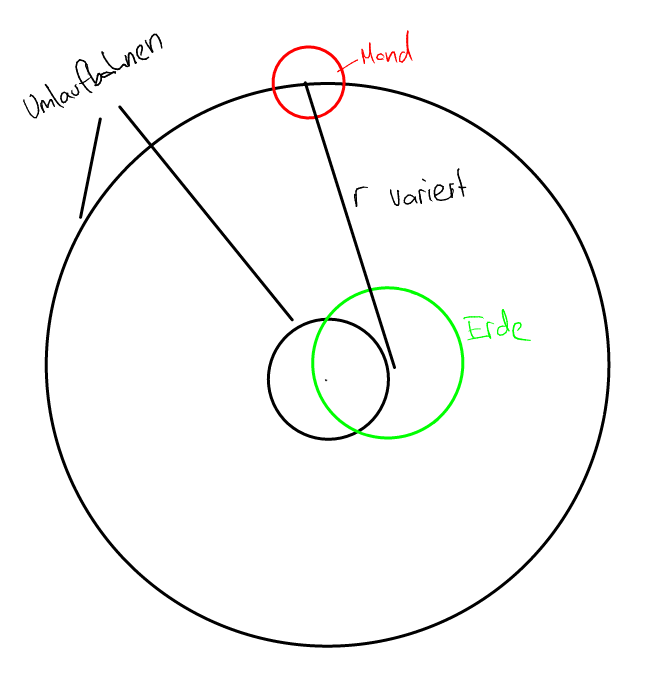
\includegraphics[width=0.5\textwidth]{radius}
	\end{figure}



	Wir haben uns folgendes überlegt:
	$$r_\text{x} = x_\text{M} - x_\text{E}$$
	$$r_\text{y} = y_\text{M} - y_\text{E}$$
	$$r = \sqrt[2]{$r_\text{x}^2 - $r_\text{y}^2}$$
	$$F_\text{x} = F_\text{E,M} \cdot \frac{r_\text{x}}{r}$$
	$$F_\text{y} = F_\text{E,M} \cdot \frac{r_\text{y}}{r}$$
	$$A_\text{xM} = \frac{F_\text{x}}{m_\text{m}}$$
	$$A_\text{yM} = \frac{F_\text{y}}{m_\text{m}}$$
	$$A_\text{xE} = \frac{F_\text{x}}{m_\text{m}}$$
	$$A_\text{yE} = \frac{F_\text{y}}{m_\text{m}}$$

	$$V_\text{xM} = \int A_\text{xM}$$

	... und so weiter für y\text{M} , x\text{E} und y\text{E}
	$$X_\text{M} = \int V_\text{xM}$$

	... und so weiter für y\text{M} , x\text{E} und y\text{E}

	Als Startwerte nehmen wir:
	$$x_\text{E0} = x_\text{M0} = y_\text{E0} = 0$$
	$$x_\text{M0} = r_\text{ME}$$

	$$v_\text{xM} = v_\text{xE} = v_\text{yE} = 0$$
	$$V_\text{yM} = 1'023 km/s$$
	\section*{Teil B}

	\section*{Teil C}

	Wir haben unser Modell aufgrund unserer Überlegungen aus Aufgabe A und B modelliert.

	\begin{figure}[h!]
			\caption{Screenshot unseres Berkeley Madonna Programms}
		    \centering
			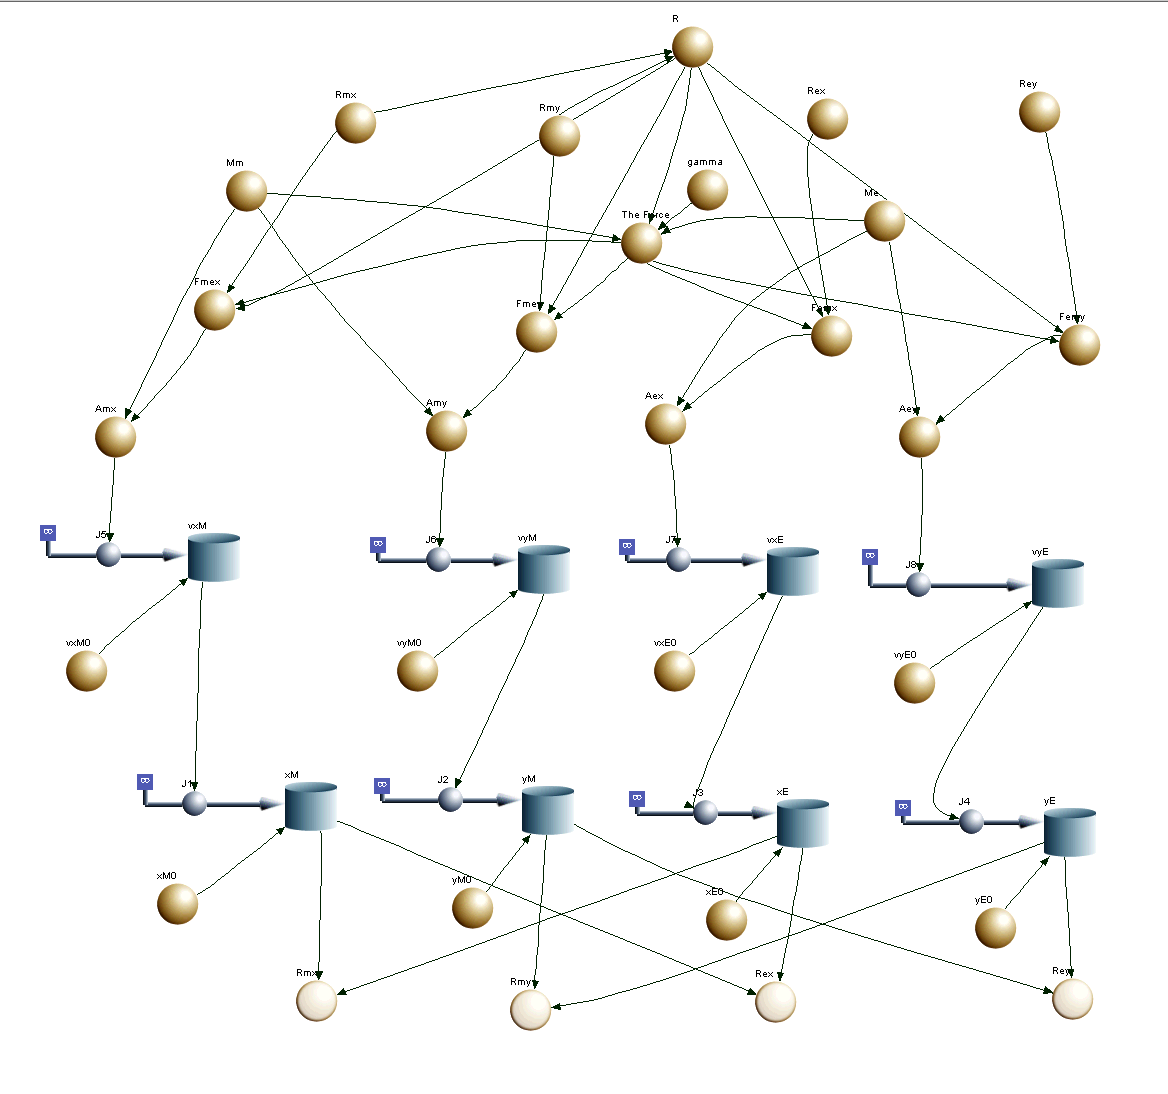
\includegraphics[width=1\textwidth]{madonna_screen}
	\end{figure}


	\begin{figure}
		\begin{tikzpicture}
			\begin{axis}[
					width=15cm, height=8cm,     % size of the image
					grid = major,
					grid style={dashed, gray!30},
					xmin=-600000000,     % start the diagram at this x-coordinate
					xmax=600000000,    % end   the diagram at this x-coordinate
					ymin=-400000000,     % start the diagram at this y-coordinate
					ymax=800000000,   % end   the diagram at this y-coordinate
				]
				\addplot table [x=a, y=b, col sep=comma, id=exp] {theforcelight.csv};
				\addplot table [x=c, y=d, col sep=comma, id=exp, red] {theforcelight.csv};
				\legend{$Mond$,$Erde$}
			\end{axis}
		\end{tikzpicture}
		\caption{Plot des CSV Files, exportiert aus Berkeley Madonna}
	\end{figure}

	Je kleiner die Zeitschritte sind, desto näher kommen sich die nummerischen Verfahren Euler, RK2 und RK4 im Resultat. Bei grösseren Zeitschritten geht die Genauigkeit beim Eulerschen Verfahren am schnellsten verloren. Schlussendlich sieht es aus als wäre die Genauigkeit wie auch der Zeitaufwand im Folgenden Schema: Euler ungenauer RK2 ungenauer RK4.
	Eigentlich hatten wir die Lösung schon längst in Berkeley Madonna, haben aber die längste Zeit nach einem Fehler gesucht der eigentlich keiner war. Das Problem war das wir im Parameter Window zu wenige Zeitschritte gemacht haben und zu früh aufgehört haben. So haben wir nie gesehen wie die eigentliche Kurve sich entwickelt hat.
	\section*{Teil D}
	Wir vermuten das sich bei einer anderen Potenz die Laufbahnen sehr schnell, sehr stark verändern würde. Da die Anziehungskraft schwächer wird (je grösser die Potenz), würde es zu ganz anderen Formen kommen, da wir gesehen haben das die Kraft "The Force" eine zentrale Rolle spielt in unserer Berechnung wie auch im Berkeley Madonna Programm.

	\bibliographystyle{ieeetr}
	\bibliography{auftrag}
\end{document}

